\documentclass[a4paper,12pt]{article} % only 10 (default), 11 and 12 pt are available

% NECESSARY PACKAGES
\usepackage[utf8]{inputenc} % to be able to use non-English characters
\usepackage{amsmath}  % improve math presentation
\usepackage{amssymb}
\usepackage{xcolor}
\usepackage{float}
\usepackage{caption} % captioning package of wonders
\usepackage{url} % to incorporate clickable links
\usepackage{cite} % takes care of citations
\usepackage[final]{hyperref} % adds hyper links inside the generated PDF file
\usepackage{placeins}
\usepackage{listings}

% NECESSARY FOR INCREASED CUSTOMIZATION PACKAGES
\usepackage{newfloat} % for defining new float in environments (e.g: figure and tables are floats)
\usepackage{graphicx} % takes care of graphic including machinery
\usepackage{tabularx} % extra features for tabular environment
\usepackage{array} % provides 'programmable' tables (cells can be tweaked much more)
\usepackage[export]{adjustbox} % to include boxed content other than figures (e.g: boxed equations)
\usepackage{wrapfig} % to make figures wrap around text
\usepackage{subcaption} % to make sub-figures inside of figures

% TWEAKS FOR PACKAGES
\usepackage[margin=2.54cm,a4paper]{geometry} % tweaks margins
\captionsetup{justification=centering} % caption justification
\captionsetup{font=12pt} % caption text size
\captionsetup{labelfont=bf} % caption label font emphasis (e.g: 'Figure X:')
\numberwithin{equation}{section} % equations are named according to their section (e.g: 2.1)
\numberwithin{figure}{section} % figures are named according to their section (e.g: 3.4)
\hypersetup{
    colorlinks=true,      % false: boxed links; true: colored links
    linkcolor=black,      % color of internal links
    citecolor=blue,       % color of links to bibliography
    filecolor=magenta,    % color of file links
    urlcolor=red          % color of website links
}

\usepackage{lipsum} % DELETE THIS AND BELOW \lipsum[]'s AND YOU'RE GOOD TO GO

%++++++++++++++++++++++++++++++++++++++++++++++++++++++++++++++++++++++++++++++++

% HERE GOES THE COVER PAGE SETUP
\newcommand{\hwcourse}{\text{Final Report}} % Title of your document
\newcommand{\hwnumber}{\text{PHYS 3266}} % Name of your study number
\newcommand{\hwdetails}{ \text{Simulating Orbital Perturbations and Inferring their Sources} \\ }
\newcommand{\hwauthor}{-Joshua Brandt- \\
                        -Paul Vollrath-  \\
} % Your name or your group's names
\newcommand{\HRule}{\rule{\linewidth}{0.5mm}} % line widths in the cover page


%++++++++++++++++++++++++++++++++++++++++++++++++++++++++++++++++++++++++++++++++

\begin{document}

% COVER PAGE IS COMPILED HERE
\begin{titlepage}

\begin{center} % Center remainder of the page
% LOGO SECTION
\includegraphics[width = 8cm]{SoPBanner.jpeg}

\\[2cm]

% HEADING SECTIONS
\textsc{\LARGE Georgia Institute of Technology}\\[.5cm]
\textsc{\Large School of Physics}\\[1.5cm]

% TITLE SECTION
\HRule \\[0.4cm]
{ \huge \bfseries \hwcourse}\\ \vspace{.5cm}
{ \huge \bfseries \hwnumber}\\ \vspace{.5cm}
{ \large \bfseries \hwname}\\ \vspace{.5cm}
{ \hwdetails}\\ \vspace{.5cm}
{ \bfseries \hwdate}\\ \vspace{.5cm}
\HRule \\[1.5cm]
\end{center}

% AUTHOR SECTION
\begin{flushleft} % left oriented author section
  \centering
    \large
    \textit{Written By:}\\
    \hwauthor% Your name
\end{flushleft}
\vspace{5cm}
\makeatletter
Date: \@date
\vfill % Fill the rest of the page with white space
\makeatother
\end{titlepage}

%++++++++++++++++++++++++++++++++++++++++++++++++++++++++++++++++++++++++++++++++


\begin{abstract}
   In this paper, we outline our code to estimate the properties of undiscovered planets by using their perterbative influence of known orbits. Using the Verlet method, we iterativley update a set of Body objects correspoding to celestial objects with new forces, velocities and positions. Each object's orbit is then analyzed to find values for its semi-major axis, eccentricity, and inclination to the ecliptic. We are able to succesfully recover eccentricities within 8.7\% excluding an outlier, semi-major axes within 0.04\% and inclinations within 0.87\% based on a four hour PACE run of our code. In our current implementation, we do not believe we have achieved the accuracy required to distinguish between error and perturbation. However, we have laid-out the first steps in the process.
\end{abstract}

\section{Introduction}

\subsubsection{History}

In 1609, Johannes Kepler formulated his three laws of orbital motion after observing the trajectory of Mars in the night-sky. His laws determine the orbits of two interacting celestial objects, allowing one to predict the size, shape, and orientation of the orbits. It wasn't until 1687 when Isaac Newton created his Universal Law of Gravity that it was understood the exact mechanism by which orbits are formed. Newton's Law, $$\vec{F}_g = \frac{Gm_1m_2}{r^2}}\hat{r}$$ now forms the basis for the analysis and prediction of orbits. With the advent of this law came the realization, which Newton made himself, that the orbits of more than two bodies is a deterministic, yet chaotic, phenomenon: there is no equivalent for Kepler's Laws for three or more bodies. This "Three-body Problem" ultimatley became the foundation for Chaos Theory.\par
There is a bright-side however. Since gravity interacts between every pair of objects, the motion of a particular object carries with it information about the distance and mass of other objects. In this way, if you know the propeties of each body graviationally interacting, you can solve Newton's Laws for each, and numerically determine its orbit. \par
This indeed became an active area of astronomical research in the mid-1800s. Ever since Uranus was observationally discovered in 1781 by William Herschel, its position in the night-sky was tracked. Astronomers John Couch Adams and Urbain Le Verrier noticed slight deviations in the orbit of Uranus: perturbations not predicted by interacting with any known planets. Using these perturbations, both astronomers calculated where a new planet would have to be to cause the observed orbit. Within the first night of looking, equipped with Le Verrier's prediction, German astronmer Johann Galle saw Neptune through a telescope for the first time. \par
Ever since that first purposeful discovery of a planet, astronomers have been using this method to detect planets, in our own Solar System and in others. In fact, many believe that there is a yet undiscovered "Planet X" outside of the Kuiper Belt beyond apparent sight. They cite unaccounted perturbations in the known planets.

\subsubsection{Goal}

The goal of our project is to computationally implement this process. Taking in a perturbed orbit, can we give an accurate suggestion of the properties of the planet doing the perturbing? The idea is to simulate a set of known planets and stars, each time making a guess as to where and how large a new planet would need to be. Evolving the system over many years, we compute properties (See \ref{sec:elements}) of the orbit, and compare them to the observed (perturbed) properties. In a sort of Bayesian analysis, if our guessed planet gives an orbit that closley matches the perturbed orbit, we can say that the guessed planet has a high likliehood of having the properties of a real planet doing the perturbing.

\subsubsection{Reference Frames}

Planetary systems in general tend to form within a plane, which in our System is called the ecliptic. More specifically, the ecliptic is the plane of the Earth-Sun orbit. As a beggining, we are analyzing the Solar System, and all subsequent discussion will be based upon that fact. \par
The ecliptic, as we will treat it, is a stationary frame: the frame in which the Earth and Sun lie in at initialization. During our simulation, we track all positions with respect to the position at which the Sun was initialized. But that is not the frame where orbital analysis typically takes place. The barycentric frame is a frame whose origin follows the center of mass of the Solar System. In order to analyze our orbits, we store the positions in this frame.

\subsubsection{Orbital Elements}
\label{sec:elements}

\begin{figure}[h!]
  \centering
  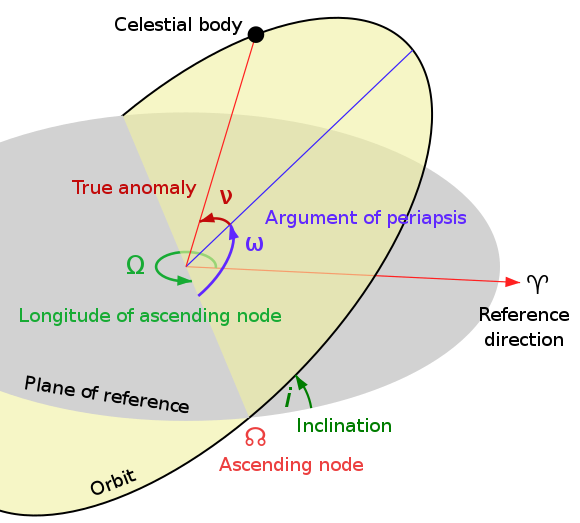
\includegraphics[scale=0.4]{OrbitalElements.png}
  \caption{A diagram of the orbital elements. From \cite{orbital_elements}}
  \label{fig:orbital_elements}
\end{figure}

Orbital elements are quantities which define the shape, size, and orientation of an orbit. Most of the elements are shown in \ref{fig:orbital_elements}, there is additionally the semi-major axis and the eccentricity. To be clear, they are:

\begin{itemize}
  \item Inclination ($\iota$) - the angle between the orbit and the ecliptic.
  \item Semi-major axis ($a$) - half of the length of the longest diameter of the ellipse.
  \item Eccentricity ($e$) - a number ranging from $0$ to $1$ quantifying how round the orbit is. $e=0$ is a circle, and $e=1$ is a line.
  \item Longitude of the Ascending Node ($\Omega$) - The angle from some reference direction to where the body passes through the ecliptic upward (the ascending node).
  \item Argument of Periapsis ($\omega$) - The angle between the ascending node and the periapsis (the point when the object is closest to what it is orbiting)
\end{itemize}


We decided to focus on the semi-major axis, eccentricity, and inclination. Those are enough to describe the shape and size of the orbit, and give a measure of how inclined it is to the ecliptic. The longitude of the ascending node and the argument of periapsis would give additional information about the orientation of the orbit and where periapsis occurs.

\section{Methods}

\subsection{Data Input}

\subsubsection{JSON Files}

The data-entry to our code is done through Javascript Object Notation (JSON) files. There are two types of JSON files that we used: a configuration file, and a planet file. An example configuration file is shown below

\begin{lstlisting}
{
  "Planets": ["Earth", "Sun", "Mercury", "Venus", "Uranus", "Jupiter",
  "Saturn", "Neptune", "Mars"],
  "dt": 3600,
  "Runtime": 60,
  "Ephemeris Date": "2001-01-10"
}
\end{lstlisting}

This contains all of the information needed to run a simulation. For each planet, the code will look for the corresponding planet file. $dt$ represents the length of the time-step to use, the Runtime is how many real seconds to fun for, and the Ephermeris Date is which date you want to initialize the Solar System at (See \ref{sec:API})). \par
The planet files contain information on the stars/planets you want to use during the simulation. Below is Earth's

\begin{lstlisting}
{
  "name": "earth",
  "mass": "<Find>",
  "iposition": "<Find>",
  "ivelocity": "<Find>",
  "Horizon ID": 399
}
\end{lstlisting}

The "\<Find\>" keyword is used when you're using a real planet which carries a unique "Horizon ID". Alternativley, you can manually enter information to make custom planets and stars. \par
The configuration file tells the code which planets to read in, and for each one it converts the information in the JSON file into an instance of our "Body" class. These bodies are manipulated by the Simulator to carry out the simulation.

\subsubsection{Horizons API \cite{Horizons}}
\label{sec:API}

Parameter values for each instance of the body class are pulled from JPL's Horizon's API. As with any API, the request is submitted by constructing a "key" URL that contains where the information is being pulled from, and the parameters of the request itself. For the Horizon API call, the commands that are manually inputed are a PlanetID, which specifies which planet the API should pull data for, and the CENTER command, which sets the reference frame with which to measure position and velocity values. Also included in the URL request are commands that specify the format of the return file, the data type desired for the return data values, and the time for which the API should pull data at. The parameters themselves are stored in the object JSON files, and are pulled from there each times the API is called. The full construction of the URL in Python 3 is shown below.

\begin{verbatim}
    url = "https://ssd.jpl.nasa.gov/api/horizons.api?"
    url += "format=json&EPHEM_TYPE=VECTORS&OBJ_DATA=YES&CENTER='500@0'"
    url += "&COMMAND='{}'&START_TIME='{}'".format(planetID, start_time, stop_time)
\end{verbatim}

Using this constructed URL, our program makes the API call, and returns a JSON file which contains a string with the request settings, and a string of the requested data. This string data is then parsed through using string methods to find the initial position and velocity, as well as the mass. Each objects JSON file is then updated with this data to then later be used in the simulator module.

\subsubsection{The Body Class}
Once all of the information about an object is known from either JSON data entry or the Horizons API, the code creates an instance of the Body class for each object participating in the simulation. Bodies have attributes including: mass, position, velocity, net force, kinetic energy which are used during the simulation; position and velocity histories which are lists storing all of the past positions of that body in the barycentric frame for later use; and semimajor axis, semiminor axis, inclination, and eccentricity which are set after the orbit is analyzed. Their methods include: adding force, removing force, and setting position \& velocity. Body objects follow through each step of the code: created at the beggining, manipulated during the simulation, and analyzed after; the code takes in the raw material and produces the product in the form of Body classes.

\subsection{Simulating Orbits}
[Talk about code]

\subsubsection{Verlet Method}
Very early on in the drafting process, it was determined that our code would be run for an extended runtime, potentially even thousands of years of simulated time. For that reason, we replaced the Euler Method in our code to implement the Verlet Method instead. This addressed several issues that we had in the earlier drafts of our program. With the Euler Method, every planet was slowly drifting out of orbit, spiraling away from the Sun. In many iterations, Mercury was eventually even slung out of orbit. To prevent this, and this build a simulator that maintained orbits that were stable in time, we replaced the Euler Method with the Verlet Method, which makes use of parallel velocity values at half-integer time steps rather than at full time steps to maintain a solution that avoids accumulating errors and is stable in time. The governing equations for this method are shown below.

\begin{equation}
\centering
x(t+h)=x(t)+hv(t+\frac{1}{2}h)
\end{equation}

\begin{equation}
\centering
k=hf(x(t+h),t+h)
\end{equation}

\begin{equation}
\centering
v(t+\frac{3}{2}h)=v(t+\frac{1}{2}h) + k
\end{equation}

We implement the Verlet Method computationally by storing an attribute in each object instance for the velocity at half time-step intervals. Since the values we want to actually store for velocity in the object velocity history attribute are at full time steps, the simulator module first updates the position value for each planet using the velocity value that is a half time-step ahead of the position value. The velocity at that full time-step is then calculated from the half time-step velocity using a Euler approximation, and stored in the velocity history object attribute. In essence, while the stored velocity values for each iteration are calculated using a Euler approximation, the generated information is calculated using the Verlet Method, and so energy is conserved over time. The accuracy of this method over time is demonstrated in the Results section.

\subsection{Orbit Analyzer}

The job of the orbit analyzer is to take in the position history of each planet and compute the orbital elements. We chose to focus on the inclination, the semi-major axis, and eccentricity (implictly requring the semi-minor axis). This is because these elements focus on the fundamental physical properties of the orbit, while others are more dependent on arbitrary reference directions (inclination depends on the "arbitrary" choice of the ecliptic plane, yet that choice is less arbitrary than the vernal equinox). We believe that with these few elements, we could capture significant and comparable information about the orbits. Of course, there were downsides to this choice. All planets lie roughly in the ecliptic plane, each with an inclination less than 10 degrees, and all orbits are mostly circular (save Mercury with $e=0.2$). This means that in two of the orbital elements, we expect to see barley any deviation, yet the semi-major axis obviously varies widley. It would then perhaps make sense to weight the semi-major axis more highly as a comparative measure: that is the dominant discriminating factor.

\subsubsection{Inclination}

The inclination $\iota$ is the tilt of an orbit with respect to the ecliptic plane; by definition, Earth has $\iota = 0$. The way we computed the inclination first involved fitting a plane to the orbit in question. The goal is to find the coefficients of the form $$Ax + By + Cz = D$$ We can do some simplification given that the Sun is necessarily in the plane of each orbit (Kepler's First Law) and the Sun is (very nearly) at $(0,0,0)$. So we know $D = 0$. Letting $C=1$ without loss of generality simplifies the problem to just finding $A$ and $B$ such that $$Ax + By = -z$$ Each orbit is stored in the form of $n$ coordinates, so constructing $$A = \begin{bmatrix}
   x_1 & y_1 &} \\
   \vdots  & \vdots  \\
   x_n & y_n}
 \end{bmatrix}\  \enspace    \vec{x}=\begin{bmatrix}A \\ B}\end{bmatrix} \   \enspace   \vec{b} = \begin{bmatrix}z_1 \\ \vdots \\ z_n}\end{bmatrix}$$
We can solve for $\vec{x}$ using least squares $$A^TA\vec{x}=A^T\vec{b}$$ utilizing numpy's method to obtain the plane. \par
We know the normal vector to the ecliptic is $n=<0, 0, 1>$ and the normal vector of the orbit's plane is $<A, B, 1>$. The inclination is simply the angle between these two vectors $$\cos(\iota)=\frac{<0, 0, 1> \cdot <A, B, 1>}{\sqrt{(A^2 + B^2 + 1)}}=\frac{1}{\sqrt{(A^2 + B^2 + 1)}}$$


\subsubsection{Semi-major Axis}

The semi-major axis for an inclined orbit is difficult to calculate since an ellipse must be fitted to data outside of the $x$-$y$ plane. To make the problem simpler, we first apply a transformation to the data to put it all in the $x$-$y$ plane. To do this, we re-write each coordinate in terms of a basis where the plane of the orbit is the new $x$-$y$ plane, whose normal vector becomes the new $z$ direction. To accomplish this, we first need the normal vector to the orbital plane (which we have from the previous section), and two linearly independent vectors in the plane of the orbit. Since we have an analytic expression for the plane, this is simple to do analytically as well. All we need to do is to rewrite the plane in vector-parametric form, as the two-dimensional span of the vectors in question, always orthogonal to the normal (which we already know).

$$x = -\frac{B}{A}y - \frac{1}{A}z$$

$$\begin{bmatrix}
   x \\
   y  \\
   z}
 \end{bmatrix} \cdot \vec{n}  = 0 \implies \begin{bmatrix}
    -\frac{B}{A}y - \frac{1}{A}z \\
    y  \\
    z}
  \end{bmatrix} \cdot \vec{n} = 0 \implies \left(\begin{bmatrix}
     -\frac{B}{A} \\
     1  \\
     0}
   \end{bmatrix}y +  \begin{bmatrix}
      -\frac{1}{A} \\
      0  \\
      1}
    \end{bmatrix}z\right)\cdot \vec{n} = 0 $$

Which gives our new basis as the column space of the transition matrix $$\begin{bmatrix}
   -\frac{B}{A} & -\frac{1}{A}} & A \\
   1 & 0 & B  \\
   0 & 1 & 1}
 \end{bmatrix}$$

Since it is best practice to use an orthonormal basis, we did this by applying the $QR$ decomposition to the transition matrix, where the column space of $Q$ is an orthonormal basis of the column space of the transition matrix.

$$\begin{bmatrix}
   -\frac{B}{A} & -\frac{1}{A}} & A \\
   1 & 0 & B  \\
   0 & 1 & 1}
 \end{bmatrix} = QR$$

With $Q$ being our orthonormal transition matrix.

The coordinates in the new basis, $\vec{x}_{\text{new}}$ is the solution of $$Q\vec{x}_{\text{new}} = \vec{x}_{\text{old}}$$
since we're expecting to transition potentially millions of points, we need a fast way of solving this system repeatedly for each new $\vec{x}_{\text{new}}$ The best way to do this is to $LU$ decompose $Q$, fulfilling the consistent row operations to create two triangular matricies which can be easily solved using Scipy's LU-Solver. So we solved $$LU\vec{x}_{\text{new}} = \vec{x}_{\text{old}}$$ for each orbit point. \par
With that done, we can know analyze the orbit within its own plane. The general equation of an ellipse $$Ax^2 + Bxy + Cy^2 + Dx + Ey + F = 0$$ can be simplified without loss of generality to $$Cy^2 + Bxy + Dx + Ey + G = -x^2$$ We solve for these coefficients the same way as before, using least squares. With these in hand, we can solve for the semi-major axis $a$ and semi-minor axis $b$ in terms of these coefficients according to $$a,b = \frac{-\sqrt{2(AE^2 + CD^2 -BDE + (B^2 - 4AC)F((A+C)\pm\sqrt{(A-C)^2 + B^2}))}}{B^2 - 4AC}$$


\subsubsection{Eccentricity}

The eccentricity is easily calculated with the standard formula $$e=\sqrt{1-\frac{b^2}{a^2}}$$

\subsection{Data Output}
Having generated the orbital parameters, the program then creates an output text file for each body object with a file name format of 

\begin{verbatim}
    object.name + "_output.txt"
\end{verbatim}

These output files, after there creation, are saved into an "OutputFiles" Folder within the project folder. To this file, the name, mass, and orbital parameters are written, followed by the listing of position history in AU. A sample file output is shown below.

\begin{verbatim}
    ----------------------------------------
    Object: Jupiter
    Mass: 1.89818722e27 kg
    Semi-Major Axis: 5.197611904 AU
    Semi-Minor Axis: 5.191180274 AU
    Eccentricity: 0.0497323818
    Rotation: -87.7953924 degrees
    Inclination: 1.3033555432 degrees
    ----------------------------------------
    Position History (x,y,z) AU
    X = 1.728  Y = 4.737  Z = -0.058
    X = 1.725  Y = 4.738  Z = -0.058
\end{verbatim}

The output module of our program also generates two graphs. The first is a set of two trajectory plots, the first including all planets, and the second only the first four planets from the Sun. These plots are created from the position history array attribute of each body object. The second graph is a plot of the energy deviations from the energy average over a specified period, visualized for the total run-time of our simulator. Both graphs are show below in the Results section.

\section{Results}

[Results]

\subsection{Errors}

[Talk about eccentricity errors]

\section{Conclusion}

[Conclusion]

\bibliography{bibliography}
\bibliographystyle{plainurl}

\end{document}

